
%(BEGIN_QUESTION)
% Copyright 2012, Tony R. Kuphaldt, released under the Creative Commons Attribution License (v 1.0)
% This means you may do almost anything with this work of mine, so long as you give me proper credit

Suppose we wished to use this DAQ unit to measure the {\it peak inverse voltage} across diode $D_3$ during operation of the power supply circuit.  Identify how we should connect channel 1 of the DAQ to do this, assuming we want the DAQ to register a {\it positive} value at the moment in time of the diode's peak inverse voltage:

$$\includegraphics[width=15.5cm]{i02120x01.eps}$$

\underbar{file i02120}
%(END_QUESTION)





%(BEGIN_ANSWER)

The phrase ``peak inverse voltage'' refers to the maximum instantaneous voltage impressed across a diode in the diode's reverse-bias (blocking) direction.  Thus, the peak we wish to capture will be positive on the cathode and negative on the anode:

$$\includegraphics[width=15.5cm]{i02120x02.eps}$$

A simpler way to manage input bias currents on the DAQ is to simply connect one of the input terminals to the DAQ ground terminal like this (although doing so may yield results a bit less precise give the unequal bias current paths to ground):

$$\includegraphics[width=15.5cm]{i02120x03.eps}$$

%(END_ANSWER)





%(BEGIN_NOTES)


%INDEX% Pictorial circuit review (analog signal wiring to data acquisition unit)

%(END_NOTES)


